% !TEX root = ../../../main.tex

\toggletrue{image}
\toggletrue{imagehover}
\chapterimage{circumference_formula}
\chapterimagetitle{\uppercase{Circumference Formula}}
\chapterimageurl{https://xkcd.com/1184/}
\chapterimagehover{Assume r' refers to the radius of Earth Prime, and r'' means radius in inches.}

\chapter{Schlüsselverteilung mit \texttt{MASSEY-OMURA}}
\label{chapter-schluesselverteilung-massey-omura}

Es war lange gar nicht klar, ob man die Idee der Schlüsselverteilung mit der Truhe sicher digital umsetzen kann. Erst in den 1970er-Jahren kamen Forscher auf die Idee, das \textbf{modulare Rechnen mit Primzahlen} zu verwenden. Daraus ergaben sich verschiedene Protokolle zur Schlüsselfestlegung. Wir stellen in diesem Kapitel ein Protokoll zur Schlüssel\textbf{verteilung} vor. Die Lernziele lauten:

\newcommand{\schluesselverteilungMasseyOmuraLernziele}{
\protect\begin{todolist}
\item Sie erklären das Protokoll \texttt{MASSEY-OMURA} und wenden es an.
\item Sie erklären, warum das Protokoll \texttt{MASSEY-OMURA} als sicher eingestuft werden kann.
\end{todolist}
}

\lernziel{\autoref{chapter-schluesselverteilung-massey-omura}, \nameref{chapter-schluesselverteilung-massey-omura}}{\protect\schluesselverteilungMasseyOmuraLernziele}

\schluesselverteilungMasseyOmuraLernziele

\section{Protokoll \texttt{MASSEY-OMURA}}

Das Protokoll \texttt{MASSEY-OMURA} wurde im Jahr 1982 von James Massey und Jim K. Omura veröffentlicht. Es kann dazu benutzt werden, um einen Schlüssel sicher von \textbf{Alice an Bob} zu \textbf{verteilen}.

\begin{example}
\label{example-massey-omura-1}
Wir verwenden $\text{key}_A$ für den Schlüssel von Alice und $\text{key}_B$ für den Schlüssel von Bob. Für den gemeinsamen Schlüssel verwenden wir $\text{key}_C$.

\begin{figure}[H]
\begin{tikzpicture}
\node at (0, 1.5) {Alice und Bob einigen sich (öffentlich) auf die Primzahl $p = 17$.};
\node[inner sep=0pt] (eve) at (0,0) {
\includegraphics[scale=0.25]{eve_tiny}};
\node[text width=2cm, align=center] (pangreifer) at (0, 1) {Eve};
\node[inner sep=0pt] (alice) at (-5,0) {
\includegraphics[scale=0.25]{alice_tiny}};
\node[text width=2cm, align=center] (sender) at (-5, 1) {Alice};
\node[inner sep=0pt] (bob) at (4,0) {
\includegraphics[scale=0.25]{bob_tiny}};
\node[text width=2cm, align=center] (empfaenger) at (4, 1) {Bob};

\node[text width=1cm, align=center, fill=black!25] (step1) at (-7, -1.25) {\Huge 1};
\node[text width=4cm, anchor=west] (step1ActionAlice) at (-6, -1.25) {$\text{key}_C = 7$ \\ $\text{key}_A = 11 \Rightarrow \text{key}_A^K = 3$};
\node[text width=3.5cm, anchor=west] (step1ActionBob) at (3, -1.25) {~\\$\text{key}_B = 9 \Rightarrow \text{key}_B^K = 9$};


\node[text width=1cm, align=center, fill=black!25] (step2) at (-7, -2.5) {\Huge 2};
\node[text width=3cm, anchor=west] (step2ActionAlice) at (-6, -2.5) {%
$\begin{aligned}
     \text{msg}_1 & = (\text{key}_C)^{\text{key}_A} \bmod p \\ 
     &= 7^{11} \bmod 17 = 14
  \end{aligned}$
};

\node[text width=1cm, align=center, fill=black!25] (step3) at (-7, -3.5) {\Huge 3};
\node[text width=2cm, anchor=west] (step3ActionBob) at (3, -3.5) {%
$\begin{aligned}
     \text{msg}_2 & = (\text{msg}_1)^{\text{key}_B} \bmod p\\ 
     &= 14^{9} \bmod 17 = 3
  \end{aligned}$
};

\node[text width=1cm, align=center, fill=black!25] (step4) at (-7, -4.5) {\Huge 4};
\node[text width=3cm, anchor=west] (step4ActionAlice) at (-6, -4.5) {%
$\begin{aligned}
     \text{msg}_3 & = (\text{msg}_2)^{\text{key}_A^K} \bmod p  \\ 
     &= 3^3 \bmod 17 = 10
  \end{aligned}$
};

\node[text width=1cm, align=center, fill=black!25] (step5) at (-7, -5.5) {\Huge 5};
\node[text width=2cm, anchor=west] (step5ActionBob) at (3, -5.5) {%
$\begin{aligned}
     \text{key}_C & = (\text{msg}_3)^{\text{key}_B^K} \bmod p \\ 
     &= 10^9 \bmod 17 = 7
  \end{aligned}$
};

\draw[-latex, very thick] ([xshift=30pt]step2ActionAlice.east) -- ([yshift=10pt]step3ActionBob.west) node[above, midway, sloped] {$\text{msg}_1 = 14$};
\draw[-latex, very thick] (step3ActionBob.west) -- ([xshift=30pt]step4ActionAlice.east) node[above, midway, sloped] {$\text{msg}_2 = 3$};
\draw[-latex, very thick] ([xshift=30pt, yshift=-10pt]step4ActionAlice.east) -- (step5ActionBob.west) node[above, midway, sloped] {$\text{msg}_3 = 10$};

\end{tikzpicture}
\caption{Eve sieht nur die drei Nachrichten $\text{msg}_1$, $\text{msg}_2$ und $\text{msg}_3$.}
\label{figure-schluesselverteilung-massey-omura-example}
\end{figure}

\end{example}

% TODO Quelle: https://its.informatik.htw-aalen.de/docs/KP/kp05-key-agreement.pdf

Das Beispiel zeigt, dass der gemeinsame Schlüssel bei Bob ankommt. Kann Eve mit den drei Nachrichten vielleicht auf den gemeinsamen Schlüssel schliessen?

\begin{important}
	Das Protokoll \textbf{Massey-Omura} ist (aus der heutigen Sicht) sicher, wenn Alice und Bob eine grosse Primzahl $p$ wählen. Eine grosse Primzahl besitzt mindestens \num{200} Dezimal\textbf{stellen}, das heisst eine Zahl mit \num{200} Ziffern! Nur dann ist gewährleistet, dass der gemeinsame Schlüssel in keiner \textbf{vernünftigen Zeit} von Eve geknackt werden kann.
\end{important}

Wir definieren nun das Schlüsselverteilungsprotokoll.

\begin{definition}[Protokoll \texttt{MASSEY-OMURA}]
Am Ende des Protokolls besitzen Alice und Bob den gemeinsamen Schlüssel $\text{key}_C$ aus $\mathbb{Z}_{p}^*$. Alle Schlüssel müssen \textbf{zufällig} gewählt werden.
\begin{itemize}
\item \textbf{Vorbereitung} (Schritt 1 in \autoref{figure-schluesselverteilung-massey-omura-ablauf})
\begin{itemize}
\item Alice und Bob einigen sich (öffentlich) auf eine Primzahl $p$.
\item Alice
\begin{enumerate}
\item[a)] Alice bestimmt den gemeinsamen Schlüssel $\text{key}_C$ aus $\mathbb{Z}_{p}^*$.
\item[b)] Alice bestimmt ihren Schlüssel $\text{key}_A$ aus $\mathbb{Z}_{p-1}^*$.
\item[c)] Alice berechnet den modularen Kehrwert $\text{key}_A^K$ zu ihrem Schlüssel $\text{key}_A$.
\end{enumerate}
\item Bob
\begin{enumerate}
\item[a)] Bob bestimmt seinen Schlüssel $\text{key}_B$ aus $\mathbb{Z}_{p-1}^*$. 
\item[b)] Bob berechnet den modularen Kehrwert $\text{key}_B^K$ zu seinem Schlüssel $\text{key}_B$.
\end{enumerate}
\end{itemize}
Die modularen Kehrwerte der Schlüssel müssen so gewählt werden, dass folgende Gleichungen erfüllt sind:
\begin{empheq}[left=\empheqbiglvert, right=\empheqbigrvert]{align*}
	(\text{key}_A \cdot \text{key}_A^K) \bmod (p-1) &= 1\\
	(\text{key}_B \cdot \text{key}_B^K) \bmod (p-1) &= 1
\end{empheq}
\item \textbf{Nachrichtenaustausch} (Schritt 2 bis 5 in \autoref{figure-schluesselverteilung-massey-omura-ablauf}) 
\begin{enumerate}
\item Alice verschlüsselt $\text{key}_C$ mit $\text{key}_A$ und erzeugt somit $\text{msg}_1$. Sie schickt $\text{msg}_1$ an Bob.
\item Bob verschlüsselt $\text{msg}_1$ mit $\text{key}_B$ und erzeugt somit $\text{msg}_2$. Er schickt $\text{msg}_2$ an Alice.
\item Alice entschlüsselt $\text{msg}_2$ mit $\text{key}_A$ und erzeugt somit $\text{msg}_3$. Sie schickt $\text{msg}_3$ an Bob.
\item Bob entschlüsselt $\text{msg}_3$ mit $\text{key}_B$ und erhält somit $\text{key}_C$.
\end{enumerate}
\begin{figure}[H]
\begin{tikzpicture}
\node at (0, 1.5) {Öffentliche Primzahl $p$.};
\node[inner sep=0pt] (eve) at (0,0) {
\includegraphics[scale=0.25]{eve_tiny}};
\node[text width=2cm, align=center] (pangreifer) at (0, 1) {Eve};
\node[inner sep=0pt] (alice) at (-5,0) {
\includegraphics[scale=0.25]{alice_tiny}};
\node[text width=2cm, align=center] (sender) at (-5, 1) {Alice};
\node[inner sep=0pt] (bob) at (4,0) {
\includegraphics[scale=0.25]{bob_tiny}};
\node[text width=2cm, align=center] (empfaenger) at (4, 1) {Bob};

\node[text width=1cm, align=center, fill=black!25] (step1) at (-7, -1.25) {\Huge 1};
\node[text width=4cm, anchor=west] (step1ActionAlice) at (-6, -1.25) {$\text{key}_C$ \\ $\text{key}_A, \text{key}_A^K$};
\node[text width=3.5cm, anchor=west] (step1ActionBob) at (3, -1.25) {~\\$\text{key}_B, \text{key}_B^K$};


\node[text width=1cm, align=center, fill=black!25] (step2) at (-7, -2.5) {\Huge 2};
\node[text width=3cm, anchor=west] (step2ActionAlice) at (-6, -2.5) {%
$\begin{aligned}
     \text{msg}_1 & = (\text{key}_C)^{\text{key}_A} \bmod p
  \end{aligned}$
};

\node[text width=1cm, align=center, fill=black!25] (step3) at (-7, -3.5) {\Huge 3};
\node[text width=2cm, anchor=west] (step3ActionBob) at (3, -3.5) {%
$\begin{aligned}
     \text{msg}_2 & = (\text{msg}_1)^{\text{key}_B} \bmod p
  \end{aligned}$
};

\node[text width=1cm, align=center, fill=black!25] (step4) at (-7, -4.5) {\Huge 4};
\node[text width=3cm, anchor=west] (step4ActionAlice) at (-6, -4.5) {%
$\begin{aligned}
     \text{msg}_3 & = (\text{msg}_2)^{\text{key}_A^K} \bmod p
  \end{aligned}$
};

\node[text width=1cm, align=center, fill=black!25] (step5) at (-7, -5.5) {\Huge 5};
\node[text width=2cm, anchor=west] (step5ActionBob) at (3, -5.5) {%
$\begin{aligned}
     \text{key}_C & = (\text{msg}_3)^{\text{key}_B^K} \bmod p
  \end{aligned}$
};

\draw[-latex, very thick] ([xshift=30pt]step2ActionAlice.east) -- ([yshift=10pt]step3ActionBob.west) node[above, midway, sloped] {$\text{msg}_1$};
\draw[-latex, very thick] (step3ActionBob.west) -- ([xshift=30pt]step4ActionAlice.east) node[above, midway, sloped] {$\text{msg}_2$};
\draw[-latex, very thick] ([xshift=30pt, yshift=-10pt]step4ActionAlice.east) -- (step5ActionBob.west) node[above, midway, sloped] {$\text{msg}_3$};

\end{tikzpicture}
\caption{Die drei Nachrichten werden öffentlich verschickt.}
\label{figure-schluesselverteilung-massey-omura-ablauf}
\end{figure}
\end{itemize}

\end{definition}

\subsection{Aufgaben}

% TODO: check evtl. überarbeiten

\begin{enumerate}
	\item Führen Sie das Protokoll \texttt{MASSEY-OMURA} für $\mathbb{Z}_{17}^*$ aus. Alice wählt $\text{key}_C = 13$. Dann wählt Alice $\text{key}_A = 5 \in \mathbb{Z}_{16}^*$ und Bob wählt $\text{key}_B = 15 \in \mathbb{Z}_{16}^*$. Notieren Sie alle Berechnungsschritte und skizzieren Sie den Ablauf der Kommunikation. Gehen Sie wie folgt vor:
	\begin{enumerate}
	\item Notieren Sie die Menge $\mathbb{Z}_{p}^*$ für $p = 17$, das heisst: $\mathbb{Z}_{17}^*$.
	\item Notieren Sie die Menge $\mathbb{Z}_{p-1}^*$ für $p = 17$, das heisst: $\mathbb{Z}_{16}^*$.
	\item Bestimmen Sie $\text{key}_A^K$ und $\text{key}_B^K$.
	\item Wenden Sie das Protokoll an und zeichnen Sie den Ablauf wie in \autoref{figure-schluesselverteilung-massey-omura-example}.
	\end{enumerate}
	
	\fillwithgrid{\stretch{1}}
	
	\newpage
	
	\item Alice und Bob wählen $p = 31$ (eine Primzahl). Führen Sie das Protokoll \texttt{MASSEY-OMURA-SCHEMA} aus. Wählen Sie die passenden Schlüssel. Notieren Sie alle Berechnungsschritte. Skizzieren Sie den Ablauf der Kommunikation. Sie können die Zahlen aus \autoref{table-modulare-kehrwerte-z30} verwenden.

\begin{table}[htb]
\centering
\begin{tabular}{|c|c|c|c|c|c|c|c|c|}
\hline
$a$                         & $1$ & $7$  & $11$ & $13$ & $17$ & $19$ & $23$ & $29$ \\ \hline
$b$ & $1$ & $13$ & $11$ & $7$ & $23$ & $19$ & $17$ & $29$ \\ \hline
\end{tabular}
\caption{Elemente aus $\mathbb{Z}_{30}^*$ und die modularen Kehrwerte.}
\label{table-modulare-kehrwerte-z30}
\end{table}

\fillwithgrid{\stretch{1}}
	
	\newpage

	\item Alice und Bob wählen $p = 113$ (eine Primzahl). Alice wählt für $\text{key}_A = 47$ und Bob wählt für $\text{key}_B = 61$. Bestimmen Sie einen gemeinsamen geheimen Schlüssel $\text{key}_C$ und führen Sie dann das Protokoll \texttt{MASSEY-OMURA-SCHEMA}. Skizzieren Sie den Ablauf und notieren Sie die Berechnungen. Berechnen Sie die modularen Kehrwerte mithilfe einer Website.
\end{enumerate}

\fillwithgrid{\stretch{1}}
	
	\newpage

\section{Kryptoanalyse Teil 1}

Beim Protokoll \texttt{MASSEY-OMURA} tauschen Alice und Bob drei Nachrichten aus. Gemäss dem Prinzip von Kerkhoff kennt Eve den Ablauf des Protokolls und kann eine Kopie jeder Nachricht erhalten. Nun steht Eve vor folgenden vier Gleichungen:
\begin{empheq}[left=\empheqbiglvert, right=\empheqbigrvert]{align*}
	\text{msg}_1 & = (\text{key}_C)^{\text{key}_A} \bmod p \\
	\text{msg}_2 & = (\text{msg}_1)^{\text{key}_B} \bmod p \\
	\text{msg}_3 & = (\text{msg}_2)^{\text{key}_A^K} \bmod p \\
	\text{key}_C & = (\text{msg}_3)^{\text{key}_B^K} \bmod p
\end{empheq}
Eve kennt nur $p$, $\text{msg}_1$, $\text{msg}_2$ und $\text{msg}_3$. Die Werte für $\text{key}_A$, $\text{key}_B$ und $\text{key}_C$ sind Eve nicht bekannt. Auch die modularen Kehrwerte kennt Eve nicht. Kann Eve das Protokoll trotzdem knacken?

\begin{example}
Wir nehmen die Rolle von Eve ein und versuchen das Protokoll \texttt{MASSEY-OMURA} für die Nachrichten aus \autoref{example-massey-omura-1} zu knacken. Wir tun hier so, als wüssten wir die Zahlen für die Schlüssel nicht. Eve hat also nur folgende Informationen:
\begin{empheq}[left=\empheqbiglvert, right=\empheqbigrvert]{align}
	14 & = (\text{key}_C)^{\text{key}_A} \bmod 17 \\
	3 & = (14)^{\text{key}_B} \bmod 17 \label{eq2} \\
	10 & = (3)^{\text{key}_A^K} \bmod 17 \label{eq3} \\
	\text{key}_C & = (10)^{\text{key}_B^K} \bmod 17
\end{empheq}
\autoref{eq2} und \autoref{eq3} haben nur eine Unbekannte. Wir fokussieren uns deshalb auf \autoref{eq2}. Da die Gleichung den Modulo-Operator beinhaltet, können wir nicht wie gewöhnlich die Gleichung umformen und den Logarithmus benutzen. Wir wissen jedoch, dass $\text{key}_B \in \mathbb{Z}_{17-1}^* = \mathbb{Z}_{16}^* = \{1, 3, 5, 7, 9, 11, 13, 15\}$ gilt. Wir müssen also nur acht Zahlen ausprobieren:
\begin{align*}
(14)^{1} \bmod 17 & = 14 \bmod 17 = 14 \neq 3 \\
(14)^{3} \bmod 17 & = \num{2744} \bmod 17 = 7 \neq 3 \\
(14)^{5} \bmod 17 & = \num{537824} \bmod 17 = 12 \neq 3 \\
(14)^{7} \bmod 17 & = \num{105413504} \bmod 17 = 6 \neq 3 \\
(14)^{9} \bmod 17 & = \num{20661046784} \bmod 17 = 3 \Rightarrow \text{key}_B = 9  \\
\end{align*}
\end{example}

%\subsection{Aufgaben}
%
%\begin{enumerate}
%\item Knacken Stufe 1
%\item Knacken Stufe 2
%\item Knacken Stufe 3
%\item Knacken Stufe 4 mit Website (\url{https://www.alpertron.com.ar/DILOG.HTM})
%\end{enumerate}

\begin{figure}[htb]
	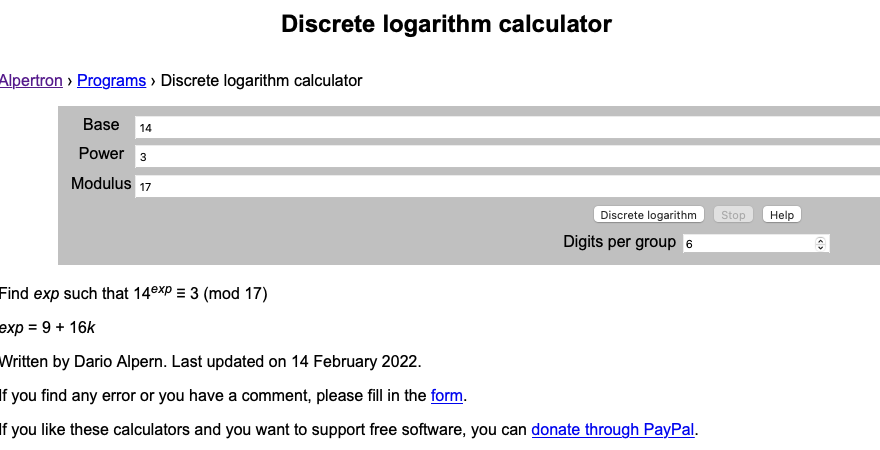
\includegraphics[scale=0.45]{dlp_solver_website_cut}
	\caption{Die Website gibt das Ergebnis in der Form $exp = 9 + 16k$ aus. Dies bedeutet, dass der gesuchte Exponent (in unserem Fall $\text{key}_B$) den Wert $9$ besitzt oder $9$ plus ein Vielfaches von $16$ (deshalb $+ 16k$).}
	\label{figure-dlp-solver-example}
\end{figure}

\newpage


\section{Kryptoanalyse Teil 2}

Wir haben im vorherigen Abschnitt und den vorherigen Aufgaben gesehen, dass Eve $\text{key}_B$ herausfinden kann. Daraus kann Eve auch $\text{key}_B^K$ berechnen. Nach dem gleichen Prinzip kann Eve auch die anderen Informationen herausfinden.

\begin{center}
	Ist das Protokoll \texttt{MASSEY-OMURA} nun unsicher?
\end{center}

Um diese Frage zu beantworten, kommt es drauf an, wie wir die Primzahl $p$ wählen. Für Primzahlen mit \num{100} bis \num{200} Stellen ergeben sich sehr grosse Zahlen für $\text{key}_A$ und $\text{key}_B$. Dann ist es ausserordentlich schwer von $\text{msg}_2 = (\text{msg}_1)^{\text{key}_B} \bmod p$ auf den unbekannten Schlüssel $\text{key}_B$ zu schliessen. 

\begin{example}
\label{example-primzahl-1}
Beispiel für eine Primzahl mit \num{232} Stellen: 12193448583342869326963419091957961
095266573861542513280292736561757668709803065055845773891258608267152015472257940
729358832588680364332872179947215421991481828415058004331484108696835906593468476
59519108393837414567892730579162319
\end{example}

Typischerweise werden in der Praxis Primzahlen in der Grössenordnung von \autoref{example-primzahl-1} benutzt. Dann kann Eve nicht mehr in einer vernünftigen Zeit $\text{key}_B$ in der Gleichung $\text{msg}_2 = (\text{msg}_1)^{\text{key}_B} \bmod p$ bestimmen. Es gibt dafür auch \textbf{keinen Algorithmus}, welcher in \textbf{vernünftiger Zeit} $\text{key}_B$ bestimmen kann.

\subsection{Der diskrete Logarithmus}

Der diskrete Logarithmus ist das Pendant zum Logarithmus aus der Analysis. Das Wort diskret ist dabei mit ganzzahlig zu übersetzen.

\begin{definition}[Diskreter Logarithmus]
	Der diskrete Logarithmus $dlog_g(y)$ ist der kleinste Wert für $x$, sodass folgende Gleichung erfüllt wird:
	
\begin{center}
	$y = g^x \bmod p$
\end{center}

Es sind also Werte für $y$, $g$ und $p$ gegeben und nur $x$ ist unbekannt.
\end{definition}

Eve muss beim Protokoll \texttt{MASSEY-OMURA} den diskreten Logarithmus $dlog_{\text{msg}_1}(\text{msg}_2)$ bestimmen um $\text{key}_B$ zu erhalten. Man glaubt, dass es für sehr grosse Primzahlen keine effiziente Methode gibt, den diskreten Logarithmus zu bestimmen. Dies kann sich in der Zukunft ändern, aber man glaubt eher nicht, dass dies der Fall sein wird.

\begin{definition}[Diskreter-Logarithmus-Problem]
Das Berechnen von $dlog_g(y)$ ist für sehr grosse Primzahlen $p$ sehr aufwendig. Bisher wurde noch kein effizienter Algorithmus für dieses Berechnung entdeckt. Wir bezeichnen es deshalb als Diskretes-Logarithmus-Problem. 
\end{definition}

Verschieben zu Schlüsselvereinbarung nach Diffie, Hellman und Merkle.

Diffie, Hellman und Merkle erkannten das Potenzial des diskreten Logarithmus und nutzen dies für die erste Entwicklung eines Schlüsselfestlegungsprotokolls. Dabei hatten Sie nicht das Ziel ein Protokoll mit perfekter Sicherheit zu erstellen, sondern eine \say{neue} Art der Sicherheit zu etablieren.

\begin{definition}[Modernes Sicherheitsverständnis]
	Ein Kryptosystem oder kryptografisches Kommunikationsprotokoll ist sicher, wenn die Kryptoanalyse so viel Zeit und Arbeit in Anspruch nimmt, dass die Kryptoanalyse in der Praxis nicht ausgeführt werden kann. Dabei darf die Art der Verschlüsselung und Entschlüsselung bekannt sein (Prinzip von Kerkhoff).
\end{definition}

Mit den Erkenntnissen von Diffie, Hellman und Merkle entstand ein völlig neuer Zweig der Kryptographie. Daraus entstanden moderne Kryptosysteme, welche zum Beispiel für elektronische Signaturen im Internet grossflächig eingesetzt werden. Wir schauen uns deshalb das Schlüsselfestlegungsprotokoll von Diffie, Hellman und Merkle an. Die damit verbundenen Konzepte wurden im Protokoll \texttt{MASSEY-OMURA-SCHEMA} aufgegriffen und eingesetzt. Das Protokoll \texttt{DIFFIE-HELLMAN-MERKLE} ist eine Alternative zum Protokoll \texttt{MASSEY-OMURA-SCHEMA} für die Schlüsselfestlegung. Es ist sogar so verbreitet, dass es gewissermassen den Standard für die Schlüsselfestlegung darstellt.